
\documentclass[11pt]{article}

\usepackage{graphicx}
\usepackage{subfigure}
\usepackage{rotating}

\begin{document}
\title{Beam-Helicity and Beam-Charge Asymmetries Associated with Deeply Virtual Compton Scattering on an Unpolarised Proton}
\author{The {\sc Hermes } Collaboration}

\maketitle

The H{\sc ermes} experiment was located on the H{\sc era} storage ring at the D{\sc esy} research centre in Hamburg, Germany. It detected the products of the 27.6\,GeV H{\sc era} lepton beam scattering from a variety of gaseous targets to help determine the structure of the target nucleon or nucleus. In this work, the results of scattering fron a hydrogen target are presented. Although the hydrogen target was sometimes polarised (i.e., the spins of the target nucleons were oriented in a specific direction with relation to the beam direction), the integrated data set has vanishing polarisation, so we say that the results are presented for an unpolarised target. This work looks in particular at asymmetries in the distribution of photons created by the scattering process where the target nucleon remains intact ($ep\rightarrow ep\gamma$); this is referred to as \emph{exclusive leptoproduction of real photons}. The results of this work are of particular interest to scientists who want to learn about the spin structure of the nucleon; the size of the asymmetries presented here can help constrain models of the way that the properties of partons in the nucleon combine to produce the properties of the nucleon itself.

\begin{figure}
\begin{center}
\subfigure[DVCS]{\includegraphics[angle=90,width=0.48\textwidth]{dvcs_both_edited}}
\subfigure[Bethe-Heitler]{\includegraphics[angle=90,width=0.48\textwidth]{bh_both_edited}}
\caption[DVCS and Bethe Heitler hand bag diagram.]{(a): The leading DVCS process in which an electron/positron ($e$) interacts with a quark in the nucleon
($N$) via a virtual photon ($\gamma^\ast$). The quark is found in the
nucleon with longitudinal momentum fraction $x+\xi$ and emits a real
photon ($\gamma$). The quark is absorbed by the nucleon with
longitudinal momentum fraction $x-\xi$. (b): The leading Bethe-Heitler process, i.e. the emission of a real photon from the incoming or outgoing lepton. This process has the same initial and final states as DVCS.}
\label{spin}
\end{center}
\end{figure}

The type of lepton used in H{\sc era} is either an electron ($e^-$) or a positron ($e^+$). By varying the beam properties, different asymmetries in the distribution of the photons can be constructed and their magnitude and sign can teach us about the partons that govern the production of the photons. In this work, the beam polarisation (i.e. the directions of the spin vectors of the beam leptons) and the beam charge were varied to produce beam-helicity and beam-charge asymmetries.

There are two physical processes that dominate the exclusive leptoproduction of real photons: Bethe-Heitler (BH) and Deeply Virtual Compton Scattering (DVCS) as shown in figure 1. In BH, the photon is produced by the beam lepton; BH contains little new information about nucleon structure within the precision available at H{\sc ermes}. In DVCS, the photon is produced by a parton in the target nucleon and these photons are the primary source of new information about nucleon structure. There are many more photons from the BH process than the DVCS process at H{\sc ermes} experimental conditions, but we can use the interference in the distributions to amplify the small contribution to the scattering amplitude from DVCS and thus gain useful information on nucleon structure by measuring asymmetries and distributions rather than absolute count rates.

\begin{figure}[ht]
\begin{center}
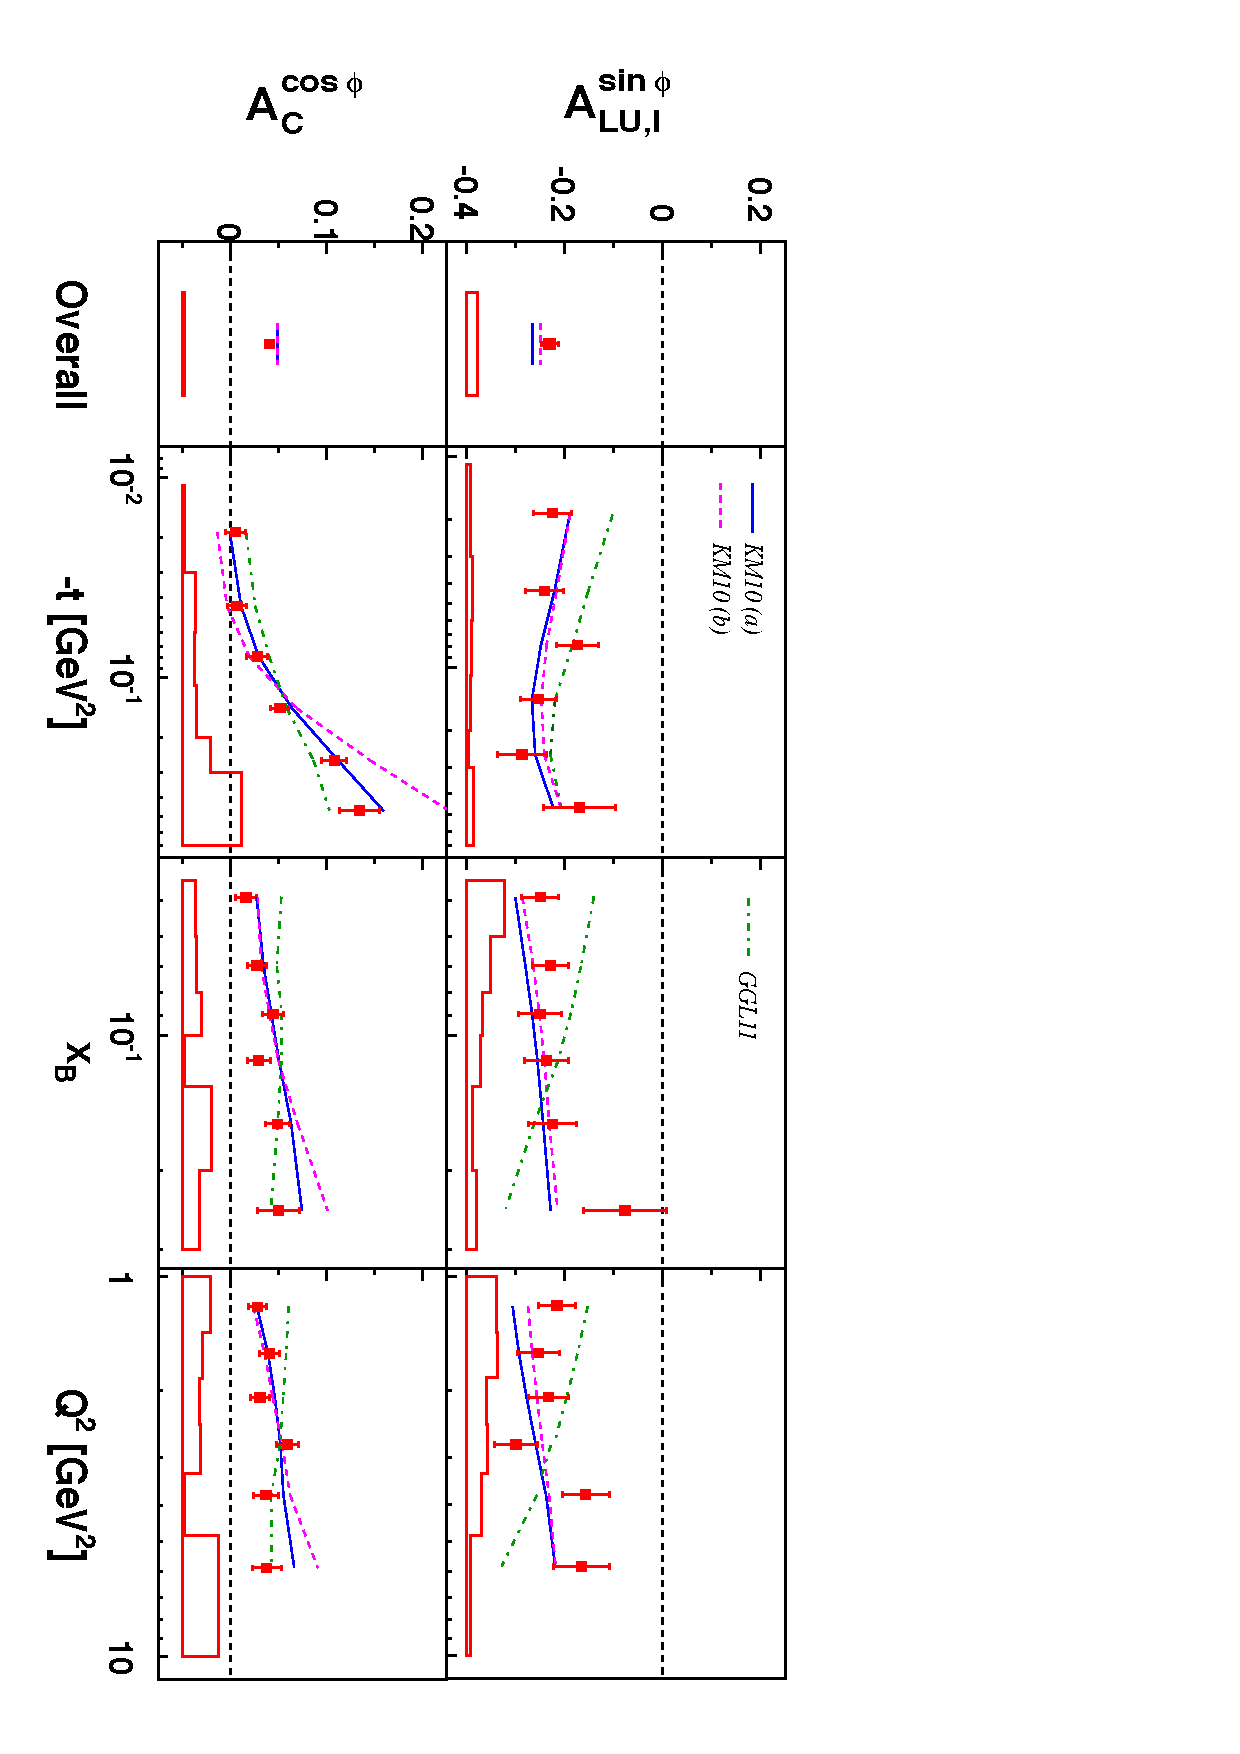
\includegraphics[angle=90,width=\textwidth]{dc90_data}
\caption{Top: The leading harmonic for the beam-helicity asymmetry as a function of three different kinematics variables for data taken throughout the lifetime of the H{\sc ermes} experiment. The amplitude seems flat across all the kinematic variables. Bottom: The leading harmonic for the beam-charge asymmetry as a function of three different kinematic variables. }
\end{center}
\end{figure}

The asymmetries in the photon distributions are measured around the azimuthal angle, which is to say that they are measured around the direction defined by the virtual photon that mediates the scattering process. The asymmetries that appear when mixing data sets of two different beam polarisations (parallel and anti-parallel to the beam direction) occur with a sinusoidal dependence. The asymmetries that appear when mixing data sets of two different beam charges (electrons and positrons) follow a co-sinusoidal dependence. We're primarily interested in the information in the leading harmonic of each term; the size of the $\sin\phi$ asymmetry amplitude and the size of the $\cos\phi$ asymmetry amplitude. In 2009, H{\sc ermes} presented results on these asymmetries from data taken in the period 1996--2005. This result builds on that previous publication and presents results on data taken over the entire lifetime of the H{\sc ermes} experiment, i.e. 1996--2007. The leading harmonics for each asymmetry are shown in figure 2. The results on this paper are the most statistically precise exclusive physics results that will be presented by H{\sc ermes} on Deeply Virtual Compton Scattering.

By comparing the sizes of these amplitudes to models that predict them, we can gain some insight to how well these models describe the structure of the nucleon. By Occam's razor, a model that predicts well many aspects of nucleon structure will likely resemble the physical truth underlying that structure. The models to which we compare the data are based on Generalised Parton Distributions (GPDs). The GPDs are multi-dimensional expansions on the familiar Parton Distribution Functions that were explored by the collider experiments at H{\sc era}. The models that are shown in figure 2 are postulated from a theoretical background and then fit to experimental data. There are two variants of the KM model that differ in the experimental data that they include. This model is postulated from first pinciples and is valid over a large kinematic range; it is fit to data from H{\sc ermes}, JLab and the colliders at H{\sc era}. The second model, GGL, is a variant of the popular phenomenological quark-diquark model that is trained to data from JLab only. The KM model fits the data better (but the data set to which it is fit includes part of the data published here).

\end{document}